\documentclass[uplatex,a4paper]{jsarticle}
\usepackage[dvipdfmx]{graphicx}
\usepackage{amsmath}
\usepackage{siunitx} %si
\usepackage[version=4]{mhchem} %ce
\usepackage{here} %for figure positioning
\usepackage{caption}
\usepackage{color}
\usepackage{booktabs, multirow}
\captionsetup{justification=centering, singlelinecheck=off}

\begin{document}

\title{Autumn Report\\誘導ラマン散乱顕微鏡を用いた脂肪トリグリセリドリパーゼ\\阻害下における中鎖脂肪酸による中性脂肪分解効果の評価}
\author{山作 百々香}
\date{\today}
\maketitle

\section{Introduction}
中性脂肪蓄積心筋血管症 (triglyceride deposit cardiomyovasculopathy; TGCV)  は2008年に平野らによって発見された疾患であり\cite{Hirano2008}、心筋や冠動脈の細胞内に中性脂肪 (triglyceride; TG) が過剰に蓄積することで、重度の心不全や動脈硬化をもたらす予後の悪い疾患である。
TGが蓄積する原因は、長鎖脂肪酸 (Long-chain fatty acid; LCFA) の細胞内代謝異常と考えられている。
図\ref{fig:normalvsTGCV}に正常な細胞とTGCV患者の細胞における脂質代謝の様子を示す。
通常、細胞内に取り込まれたLCFAはTGとして蓄積するか、ミトコンドリアに取り込まれ$\beta$酸化を介してエネルギー産生に利用される。
細胞内に蓄積したTGはエネルギー源となり、必要に応じて脂肪トリグリセリドリパーゼ (adipose triglyceride lipase; ATGL) をはじめとする細胞内のリパーゼによって加水分解され、LCFAとなって$\beta$酸化に用いられる。
これに対し、TGCV患者の細胞ではLCFAの代謝異常により、TGが分解されず過剰に蓄積する。
その結果、エネルギー不全やTGの蓄積による脂肪毒性が生じる。
LCFAの代謝異常の原因の一つとして、ATGLをコードするPNPLA2遺伝子の変異が報告されている。
しかしながら、多くの症例において遺伝的原因が明らかとなっていない。
また、TGCV患者の細胞では、LCFAの受容体およびトランスポーターであるCD36の発現が増加し、LCFAの取り込みが増えることでTGの蓄積がさらに増えることが報告されている\cite{Hirano2014}。

\begin{figure}[H]
	\centering
	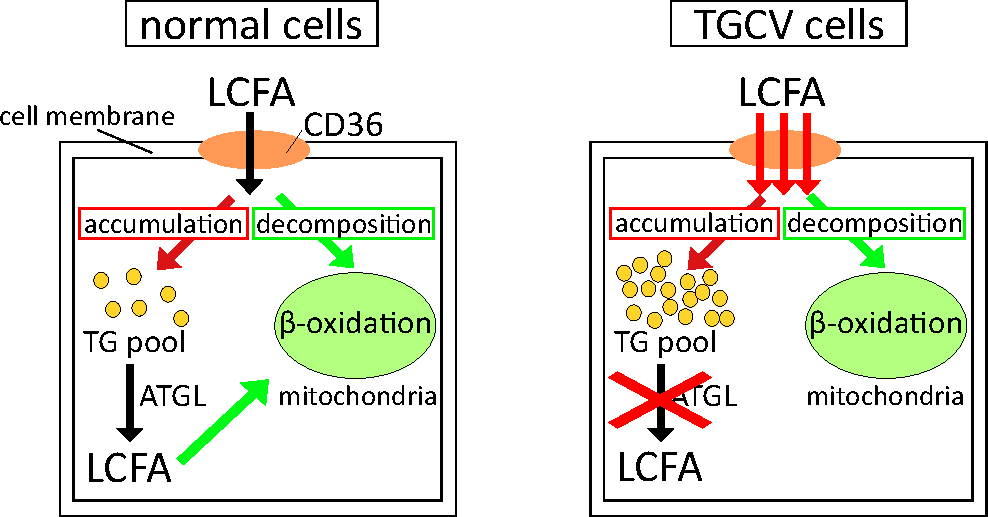
\includegraphics[width=15cm,pagebox=cropbox,clip]{figure/1_1_TGCVcell.pdf}
	\caption{正常細胞とTGCV患者の細胞における脂質代謝\\LCFA: Long-chain fatty acid、TG: Triglyceride、ATGL: Adipose triglyceride lipase \label{fig:normalvsTGCV}}
\end{figure}

TGCVの治療には中鎖脂肪酸 (medium-chain fatty acid; MCFA) の利用が有効である。
鈴木らは、TGCVを模擬したATGLノックアウトマウスにMCFAを与えることでLCFAの代謝が促進され、心筋細胞内の脂肪の蓄積が減少することを発見した\cite{Suzuki2018}。
しかしながら、MCFAがLCFAの代謝を促進するメカニズムはわかっていない。

そこで本研究では、MCFAによる脂質代謝促進効果をTGCV模擬細胞で評価することを目的とする。
評価方法としては、MCFAと重水素置換したLCFAを与えた細胞において、ATGLを阻害してTGCVの状態を模擬した後に脂肪動員を誘導し、LCFA由来のTGの分解の様子を評価する。
ここで観察には誘導ラマン散乱 (stimulated Raman scattering; SRS) 顕微鏡を用いる。
SRS顕微鏡を用いることで、重水素置換したLCFAの分布を特異的に観察し、LCFAの脂質量を測定することができる。

SRSは非線形光学効果のひとつであり、周波数$\omega_{\mathrm{p}}$のポンプ光と周波数$\omega_{\mathrm{s}}$のストークス光を分子に照射した際に、2つの光の周波数差$\omega_p-\omega_s$が分子振動の共鳴周波数と一致するとエネルギー遷移が生じ、ポンプ光が減衰しストークス光が増幅する現象である。
SRS顕微鏡では、SRS信号の強度が分子密度に比例することから分子密度を定量的に測定することが可能である。
本研究では重水素置換したLCFAをSRS顕微鏡で観察することでMCFAとLCFAを識別し、LCFAの脂質量を測定する。
炭素-重水素結合 (\ce{C-D}) の分子振動\SI{2100}{\cm^{-1}}は生体分子由来の分子振動がほとんど存在しないサイレント領域 (1800-2800 \si{\cm^{-1}}) に含まれる。
したがって重水素置換LCFA由来の信号を特異的に検出することができる。

本報告期間では、脂肪動員の透過タイムラプス観察および脂肪細胞のSRSイメージングを行った。
前者では、脂肪動員誘導剤による脂肪動員誘導効果、ATGL阻害試薬による脂肪動員阻害効果、MCFAによる脂肪動員促進効果についてそれぞれ評価した。
後者に関しては、以前修理を行ったSRS信号検出器の性能評価を行った後、脂肪細胞のSRSイメージングが可能であることを確認した。

\section{Materials \& Methods}

\subsection{サンプル調製}
\subsubsection{3T3-L1脂肪細胞への脂肪酸ロード}
サンプルには3T3-L1細胞を使用し、これを脂肪細胞に分化させた後、パルミチン酸 (C16:0) を脂肪細胞にロードした。
細胞培養、分化、脂肪酸ロードの手順を以下に示す。
図\ref{fig:FAload}には手順の概念図を示す。

\begin{enumerate}
	\item  
	3T3-L1細胞\num{5.0E4} cells/mLをガラスボトムディッシュ (D11531H、松浪硝子工業株式会社) に200 \si{\uL}播種した。
	1日後、培地を2 mL加えて培養した。
	培地はDulbecco's Modified Eagle Medium (DMEM-Low; 041-29775、和光純薬)に\SI{10}{\percent} neonatal bovine serum (NBCS; 1601067、Gibico) と\SI{1}{\percent} Penicillin-Streptomycin-amphotericin B suspension (Anti; 161-23181、和光純薬) を加えて作製した。
	培地は2日に1回交換した。\\

	\item  
	3T3-L1細胞を脂肪細胞に分化させた。
	1で培養した3T3L1細胞が\SI{80}{\percent}コンフルエントに達したら、培地を分化誘導培地に交換して2日間培養した。
	分化誘導培地は、DMEM-Lowに\SI{10}{\percent} fetal bovine serum (FBS; 092910154、MP Biomedicals)、\SI{1}{\percent} Anti、分化培地用添加試薬 (MK429、TKR; \SI{10}{\ug\per\mL} insulin、2.5 \si{\micro\mol\per\L} dexamethasone、0.5 mM 3-isobutyl-1-methylxanthine (IBMX)) を加えて作製した。
	2日間培養した後、維持培地に交換し、3日おきに培地を交換して培養した。
	維持培地はDMEM-Lowに\SI{10}{\percent} FBS、\SI{1}{\percent} Anti、10 \si{\ug\per\mL} insulin (MK429、TKR) を添加して作製した。\\

	\item  
	分化した細胞にパルミチン酸をロードした。
	まず、パルミチン酸250 \si{\micro\mol\per\L}を含む培地を作製した。
	パルミチン酸を無水アルコールで40 mMになるように調整した後、さらに10 \si{\percent} bovine serum albumin (BSA; 30 \si{\percent} BSA (017-22231、和光純薬) を3倍希釈して使用) で8倍希釈し5 mMとした。
	この脂肪酸溶液を\SI{37}{\degreeCelsius}の恒温槽で30分間撹拌した後、維持培地でさらに20倍希釈することで、最終濃度250 \si{\micro\mol\per\L}に調整した。
	次にディッシュから培地を除去し、脂肪酸を含む培地を2 mL添加して培養した。

\end{enumerate}

\begin{figure}[H]
	\centering
	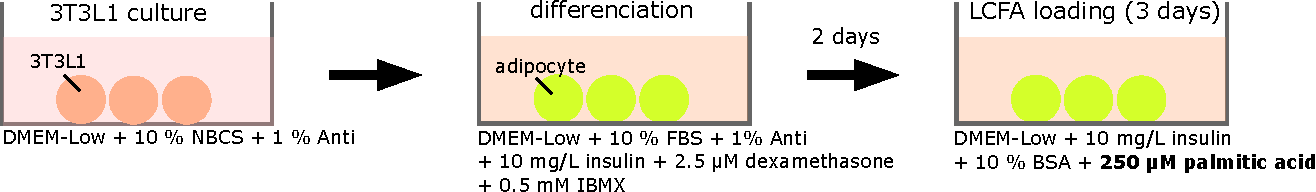
\includegraphics[width=15cm,pagebox=cropbox,clip]{figure/2_1_FAload.pdf}
	\caption{脂肪酸ロードの手順 \label{fig:FAload}}
\end{figure}

\subsubsection{脂肪トリグリセリドリパーゼの阻害}
TGCVの細胞を模擬するために、ATGLの活性を阻害した。
ATGL阻害剤として、Atglistatin (HY-15859、MedChemExpress) を使用した。
AtglistatinはATGLに特異的に作用して脂肪動員を阻害する\cite{Mayer2013}。
ATGL阻害の手順としては、まずディッシュ内の培地を除去し、HBSSで2回洗浄した後、ATGL阻害剤含有培地を加え、2時間インキュベートした。
ATGL阻害剤含有培地はDMEM-Lowに\SI{2}{\percent} BSA、Atglistatin 40 \si{\micro\mol\per\L}または50 \si{\micro\mol\per\L}を加えて作製した。
なお、HBSSおよびATGL阻害剤含有培地は使用前に\SI{37}{\degreeCelsius}に加温した

\subsubsection{脂肪動員の誘導}
脂肪細胞に脂肪動員誘導剤を与え、脂肪動員を誘起した。
ディッシュ内の染色液を除去し、HBSSで2回洗浄した後、脂肪動員誘導剤を2 mL加えて観察した。
脂肪動員誘導剤はDMEM-Lowに\SI{10}{\percent}FBS、25 mM HEPES、0.5 mM IBMX、10 \si{\micro\mol\per\L} isoproterenol (Tocris bioscience、Ellisivelle、MO、USA) を加えて作製した\cite{Hashimoto2012}。
誘導剤にBSAを添加する場合は、\SI{10}{\percent}FBSの代わりに\SI{2}{\percent}BSAを添加した\cite{Hashimoto2012}。
%\textcolor{red}{BSAを加えるだけでなく,FBSを取り除くのはどういう理由があるのでしょうか?}
ATGL阻害を行う場合は、BSAを添加した誘導剤にAtglistatinを40 \si{\micro\mol\per\L}加えた。
中鎖脂肪酸のよる脂肪分解促進効果を観察する際には、さらにオクタン酸 (C8:0)を加えた。
オクタン酸を加える際は、パルミチン酸をロードする際と同様の手順でオクタン酸を脂肪動員誘導剤に添加した。
HBSSおよび脂肪動員誘導剤は使用前に\SI{37}{\degreeCelsius}に加温した。

\subsection{透過観察システム}
脂肪動員の透過タイムラプス観察には倒立型光学顕微鏡 (ECLIPSE Ti、Nikon) を用いた。
顕微鏡の操作には画像統合ソフトウェアNIS-Elements (Nikon) を用いた。
タイムラプス観察は5分おきに撮影し、2時間撮影した。
タイムラプス観察の各撮影タイミングでステージを移動させ、ディッシュ内の複数の箇所を観察した。

\subsection{脂肪滴の体積の算出}
取得した蛍光像から脂肪滴の領域を抽出する際はImageJを使用した。
図\ref{fig:binary}に脂肪滴抽出の流れの概念図を示す。
脂肪滴抽出の手順としては、まず取得した画像のコントラストを調整した ([Image]$>$[Adjust]$>$[Brightness/Contrast])。
次に画像を白黒8 bit画像に変換 ([Image]$>$[Type]$>$[8-bit]) してから二値化 ([Image]$>$[Adjust]$>$[Threshold]) し、ノイズを除去し目的の脂肪滴を取り出すことができるように二値化の閾値を調整した。
次に粒子解析ツール ([Analyze]$>$[Analyze Particles]) を用いて面積\SI{50}{\micro\metre\squared}以上、楕円率0.5 以上の楕円を抽出し、抽出した領域の面積を算出した。
図\ref{fig:binary}に脂肪滴を含む細胞の透過像および脂肪滴の蛍光像、蛍光像から二値化した画像と抽出した領域を示す。
ImageJを用いて算出した面積から、脂肪滴を球形と仮定して、脂肪滴の半径および体積を計算した。
脂肪滴の半径は円の面積の公式 (式\eqref{square}) から算出し、体積は球の体積の公式 (式\eqref{volume}) から算出した。
式\eqref{square}、式\eqref{volume}において、$S$、$r$、$V$はそれぞれ、脂肪滴の面積、半径、体積を表す。
さらに、観察終了時間における脂肪滴の体積 ($V_{\mathrm{end}}$) と観察開始時間における体積 ($V_{\mathrm{0}}$) の比$\frac{V_{\mathrm{end}}}{V_{\mathrm{0}}}$を求め、脂肪滴の体積変化を評価した。

\begin{figure}[H]
	\centering
	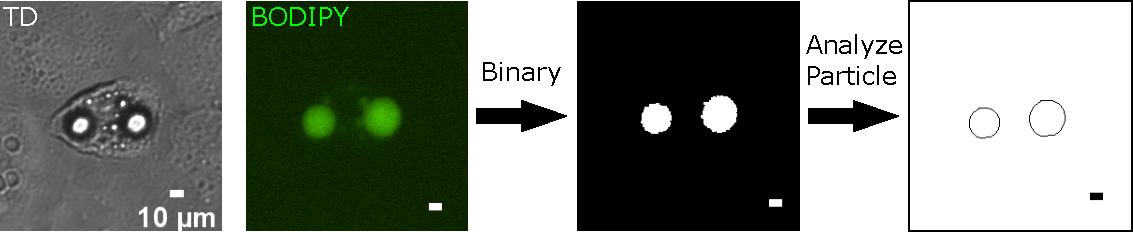
\includegraphics[width=15cm,pagebox=cropbox,clip]{figure/2_3_binary.pdf}
	\caption{蛍光像からの脂肪滴抽出	\label{fig:binary}}
\end{figure}

\begin{equation}\label{square}
	S=\pi r^2
\end{equation}

\begin{equation}\label{volume}
	V=\frac{4}{3}\pi r^3
\end{equation}

\subsection{SRS検出器の性能評価}
以前修理したSRS検出器の性能評価を行った。
図\ref{SRSdetector_cirkit}に検出器の回路図を示す。
回路には3つのLC回路で構成される、中心周波数20 MHzのバンドパスフィルターと中心周波数80 MHzのRLCバンドストップフィルターが含まれる。
20 MHzバンドパスフィルターにより入力信号に含まれるノイズを除去し、80 MHzバンドストップフィルターによりレーザーの繰り返し周波数に由来するノイズを除去して$V_{\mathrm{AC}}$にSRS信号を出力する。
また、DC出力$V_{\mathrm{DC}}$は透過観察に用いられる。

\begin{figure}[H]
	\centering
	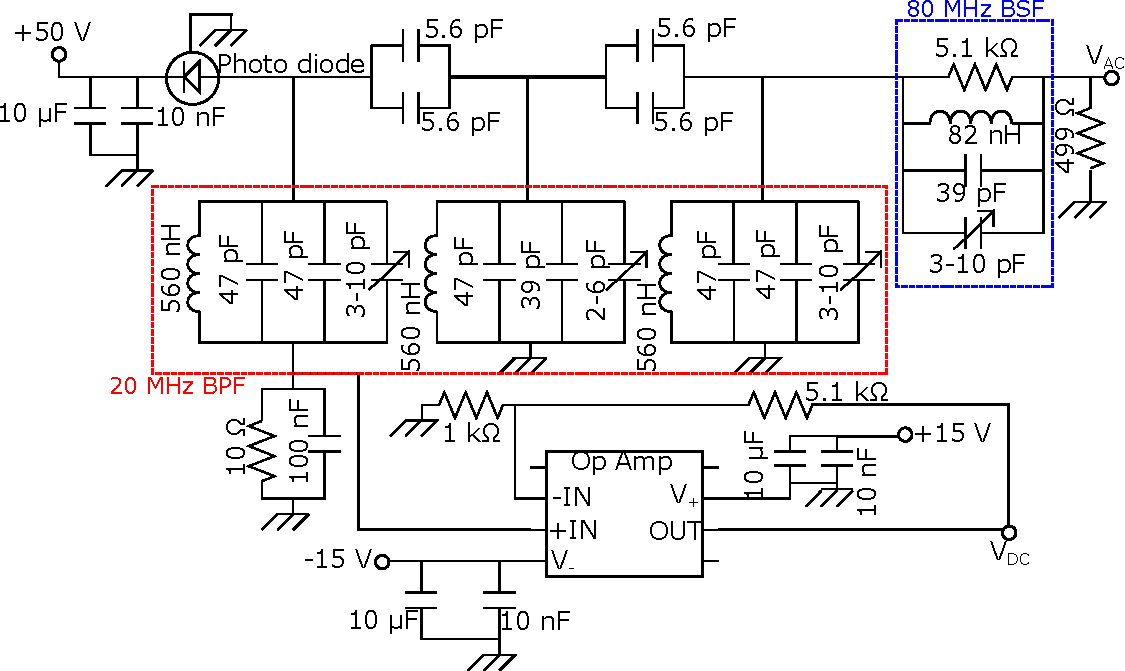
\includegraphics[width=15cm,pagebox=cropbox,clip]{figure/2_4_SRSdetector_cirkit50Vdc.pdf}
	\caption{SRS検出器の回路構成\\BPF: Band pass filter、BSF: Band stop filter	\label{SRSdetector_cirkit}}
\end{figure}

検出器に二色のレーザー光を入射し、周波数20 MHzの信号を特異的に検出できるか確認した。
性能評価に用いた光学系を図\ref{SRScheckOptsystem}に示す。
光源には、共振周波数80 MHzのピコ秒モード同期Ti:Sapphireレーザー ($\omega_{\mathrm{p}}$) と、それにacoustic optictunable filter (AOTF) を適用したもの ($\omega_{\mathrm{s}}$) を使用した。
後者のレーザー光には電気光学変調器 (electro-optic modulater; EOM) を用いて20 MHzで強度変調をかけた。
ファンクションジェネレータ (WF1948、NF) から周波数20 MHz、振幅0.3 \si{V_{\mathrm{p-p}}}の正弦波信号を出力し、アンプで増幅してEOMに印加した。
変調光と非変調光をともに倒立型顕微鏡 (ECLIPSE Ti-U、Nikon) を通して検出器に入射した。
検出器前における非変調光のパワーは16 mWとし、変調光と非変調光の強度比${I_{\mathrm{modulated}}/I_{\mathrm{non-modulated}}}$が$10^(-6)$から$10^(-2)$となるように、変調光の強度を変化させた。
変調光の強度を変化させる際はNDフィルター (ND03、ND10、ND20、ND13A、NE30A-B) を使用した。
使用したNDフィルターの組み合わせとそのときの検出器前での変調光のパワー$I_{\mathrm{modulated}}$、強度比${I_{\mathrm{modulated}}/I_{\mathrm{non-modulated}}}$を表\ref{tab:AOTFpower}に示す。
信号の検出にはロックインアンプを使用した。
検出器のAC出力を19.2-23.6 MHzバンドパスフィルタ (SBP-21.4、Mini-Circuits) に通した後、プリアンプ (SA-220F5, NF) で増幅しオシロスコープ (DRO2012、Tektronix) で測定した。
プリアンプおよび検出器のオペアンプの電源には$\pm$15 V 直流電源 (SA-915D1、NF) を用いた。
また、直流電源 (TR6143、ADVANTEST) を用いてフォトダイオードに50 Vの逆電圧を与えた。

\begin{figure}[H]
	\centering
	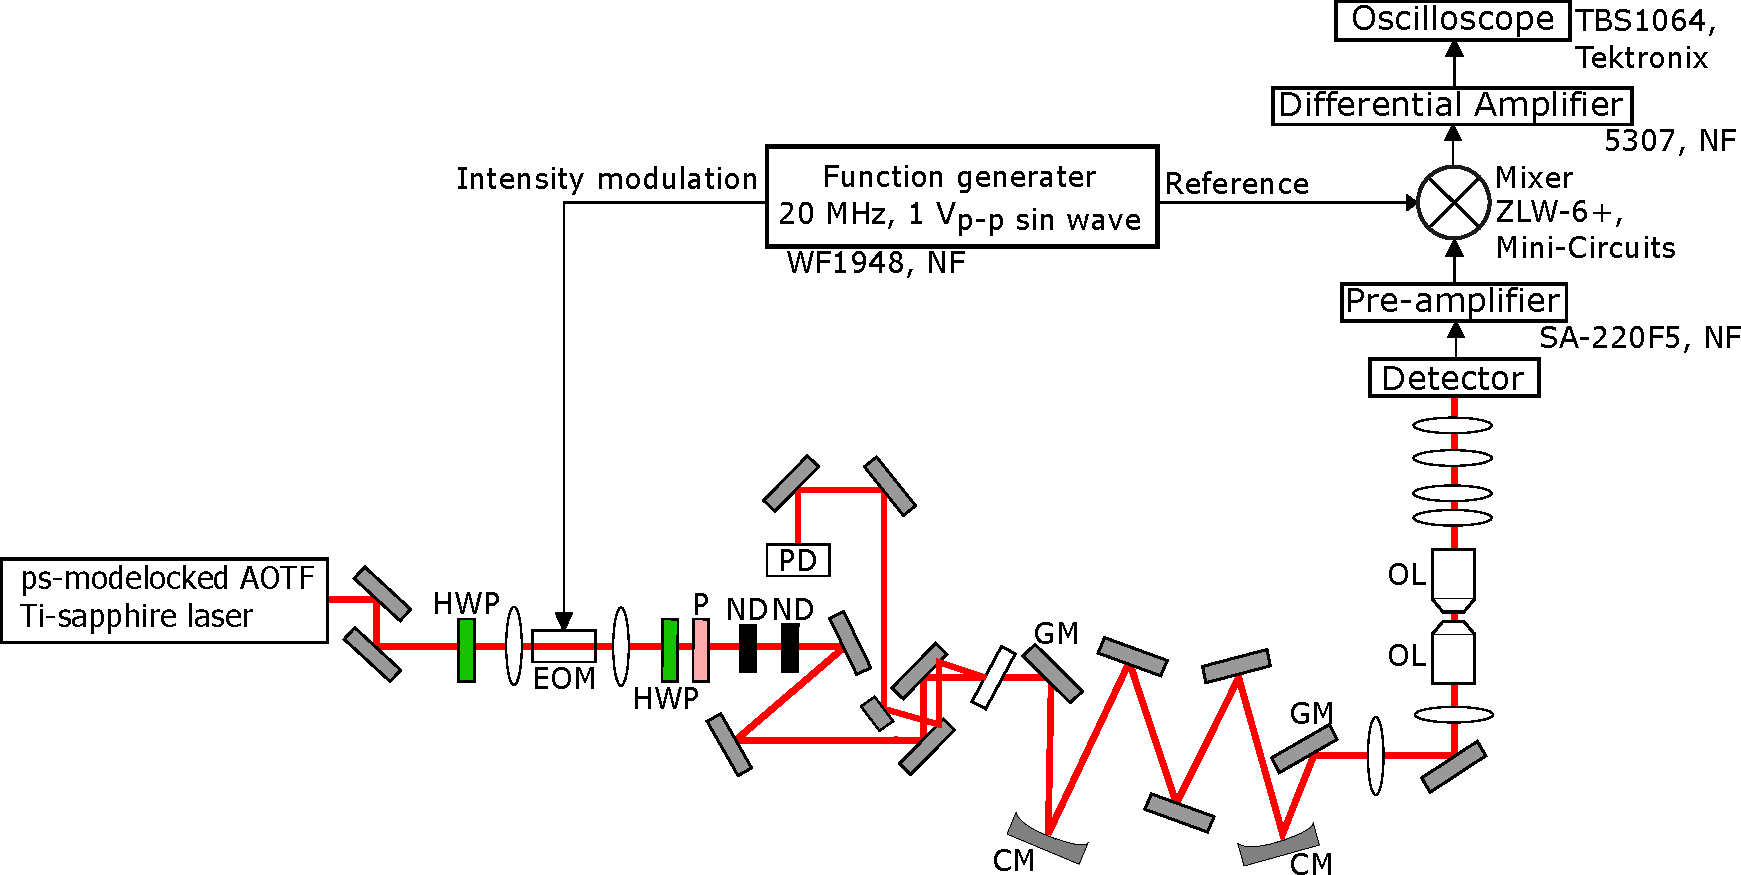
\includegraphics[width=15cm,pagebox=cropbox,clip]{figure/2_6_SRScheck_optsystem.pdf}
	\caption{検出器性能評価に用いた光学系 \\HWP: Half wave plate、P: Polarizer、ND: ND filter、BS: Beam sampler、\\GM: Galvanometric mirror、CM: Concave mirror、OL: Objective lense \label{SRScheckOptsystem}}
\end{figure}

\begin{table}
    \centering
    \caption{NDフィルター適用時の変調光のパワー}
	\label{tab:AOTFpower}
    \begin{tabular}{|c|c|c|c|c|} \toprule
        \multicolumn{2}{|c|}{\multirow{2}{*}{$I_{\mathrm{modulated}}$ / \si{\micro\watt} ($I_{\mathrm{modulated}}/I_{\mathrm{non-modulated}}$)} & \multicolumn{3}{c|}{Filter2} \\ \cmidrule{3-5}
        & & NE30A-B & NE30A-B+ND13A & NE30A-B+NE30A-B \\ \midrule 
        \multirow{6}{*}{Filter1} & None & 48.6746 & 2.81881 & 0.645092 \\ \midrule
        & ND03 & 21.9344 & 1.27025 & 0.2907 \\ \midrule
		& ND10 & 6.42011 & 0.371798 & 0.085087 \\ \midrule
		& ND03+ND10 & 2.86687 & 0.166024 & 0.037995 \\ \midrule
		& ND20 & 2.61549 & 0.151467 & 0.034664 \\ \midrule
		& ND03+ND20 & 1.18298 & 0.068508 & 0.015678 \bottomrule
    \end{tabular}
\end{table}

\subsection{SRSイメージング}

さらに、参照信号として20 MHzの正弦波信号をファンクションジェネレータからミキサーに供給した。
ミキサーを用いて入力信号に参照信号をかけた信号を出力し、この信号を差動増幅器 (5307、NF) を用いて増幅した。
なお、ミキサーから差動増幅器への信号入力は\SI{50}{\ohm}ターミネーターを介して行った。
最後に差動増幅器の出力をオシロスコープ (DRO2012、Tektronix) で測定した。

\section{Results}
\subsection{温度制御の有効性の評価}
観察時の培地の温度が脂肪動員におよぼす影響について検討した。
図\ref{fig:Lipolysis_TC}には、温度制御を行った状態と行っていない状態でそれぞれ脂肪滴のタイムラプス観察を行った結果を示す。
図\ref{fig:dV_TC}には、観察結果から求めた体積変化率を示す。
図\ref{fig:dV_TC}より、温度制御の有無に関わらず、脂肪動員誘導剤を与えることで脂肪滴の体積が有意に減少することが確認された\textcolor{red}{どういう検定使ったのか?有意水準は?}。
\textcolor{red}{温度制御の有無に関する結論は?}

\begin{figure}[H]
	\centering
	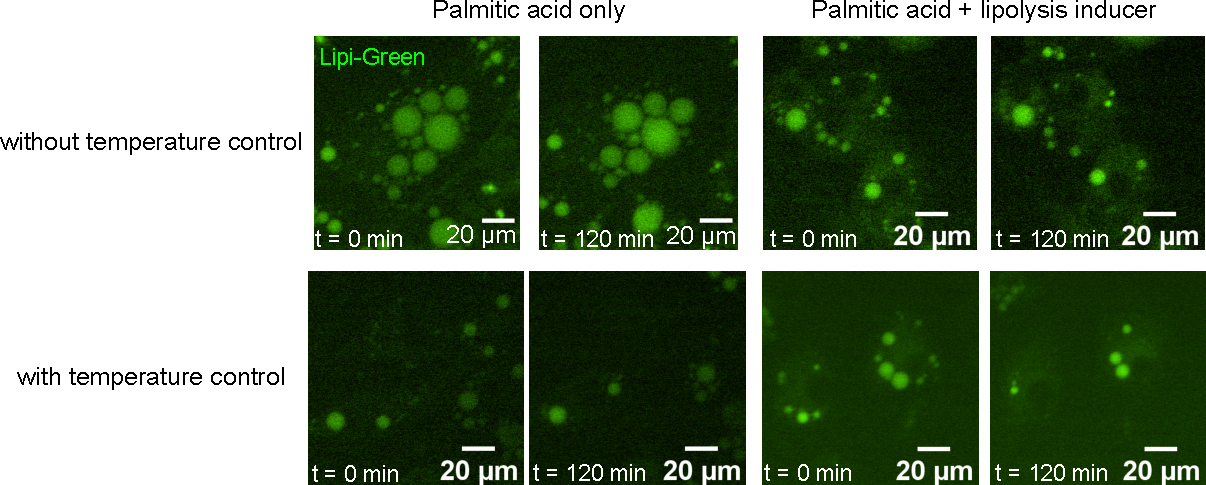
\includegraphics[width=15cm]{figure/3_1_Lipolysis_WvsWOTempCont.pdf}
	\caption{温度制御下での脂肪動員の観察結果	\label{fig:Lipolysis_TC}}
\end{figure}

\begin{figure}[H]
	\centering
	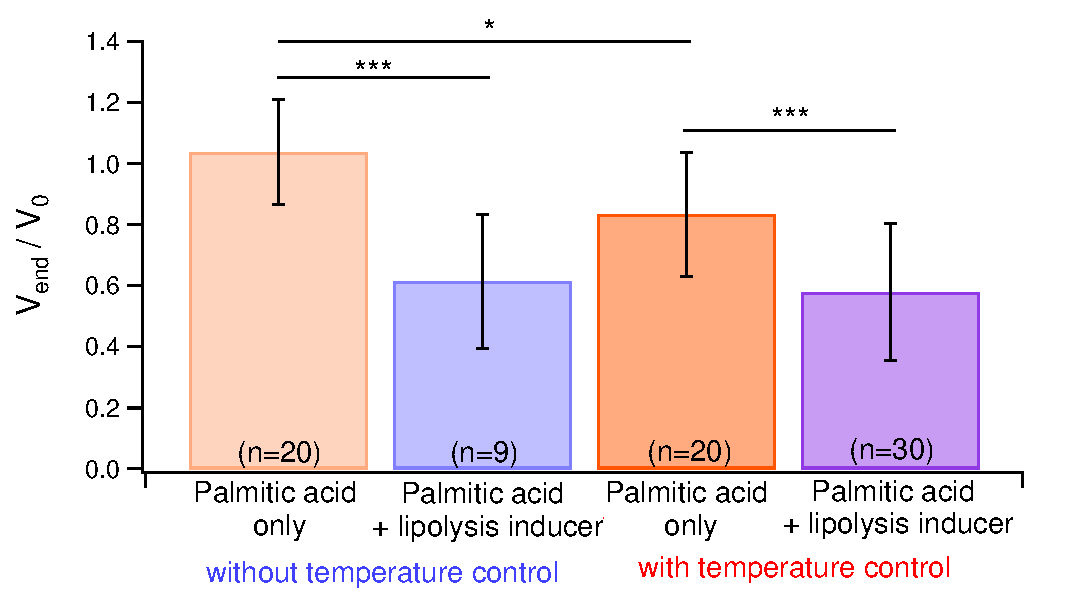
\includegraphics[width=15cm]{figure/3_2_dV_TempCont.pdf}
	\caption{温度制御を行った場合と行っていない場合の脂肪滴の体積変化	\label{fig:dV_TC}}
\end{figure}

\subsection{アルブミンの有効性の評価}
脂肪動員誘導剤にBSAを含む場合 (BSA(+)) と含まない場合 (BSA(-)) について、それぞれ脂肪動員の様子をタイムラプス観察した。
観察結果を図\ref{fig:Lipolysis_BSA}に示す。
図\ref{fig:Lipolysis_BSA}より、BSAの有無による脂肪滴の体積変化の違いは小さいと考えられる。
\textcolor{red}{なんでアルブミンの有効性を確認する必要があると考えているのかが書かれていない}

\begin{figure}[H]
	\centering
	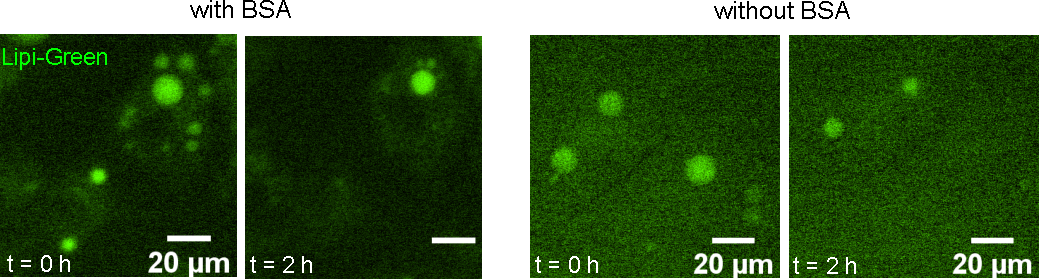
\includegraphics[width=15cm]{figure/3_3_WorWOBSA.pdf}
	\caption{BSAを与えた場合と与えていない場合の脂肪動員の観察結果	\label{fig:Lipolysis_BSA}}
\end{figure}

\subsection{ATGL阻害剤による脂肪動員阻害効果の確認}
ATGL阻害剤を与えた場合と与えていない場合でそれぞれ脂肪動員を誘導し、脂肪動員の観察を行った。
観察結果を図\ref{fig:ATGLiMCFATest}に示す。
図\ref{fig:ATGLiMCFATest}より、ATGL阻害剤を与えずに脂肪動員を誘導した場合には脂肪滴の体積が顕著に減少するのに対して、ATGL阻害剤を投与した場合には脂肪滴の体積がほとんど変化していない。
この結果から、ATGL阻害剤によって脂肪動員が阻害されることを確認できた\textcolor{red}{定量的な評価は?}。

\begin{figure}[H]
	\centering
	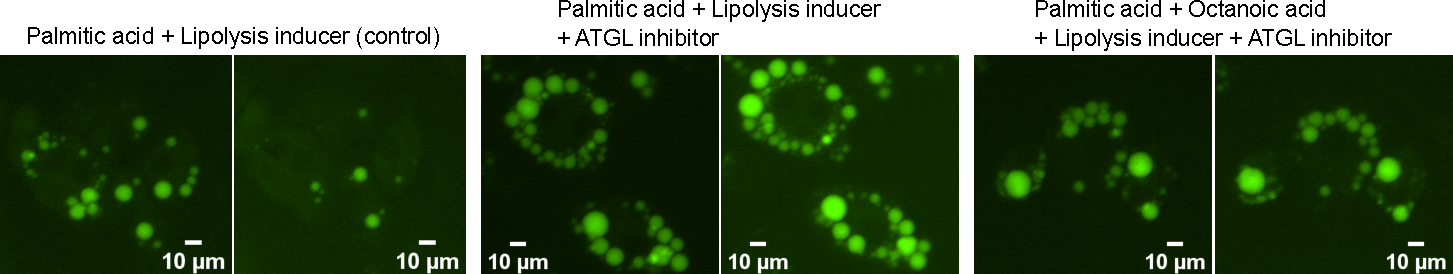
\includegraphics[width=15cm]{figure/3_4_ATGLi_MCFA.pdf}
	\caption{脂肪動員誘導剤、ATGL阻害剤、中鎖脂肪酸を与えた際の脂肪動員の観察結果	\label{fig:ATGLiMCFATest}}
\end{figure}

\subsection{中鎖脂肪酸による脂肪動員促進効果の検証}
パルミチン酸とともにオクタン酸をロードした脂肪細胞において、ATGL阻害下で脂肪動員を誘導した際の脂肪滴の体積変化を観察した。
図\ref{fig:ATGLiMCFATest}に観察結果を示す。
オクタン酸を与えた場合と与えていない場合で、脂肪滴の体積変化の様子に違いは見られず、いずれも体積がほとんど変化していなかった\textcolor{red}{定量的な評価は?}。

\subsection{SRS検出器の動作確認}
まず、LEDを用いてSRS検出器の動作確認を行った。
図\ref{fig:DetectorTest_LED}にLEDへの入力信号の周波数$f_{\mathrm{in}}$を10 MHzから100 MHzまで変化させた際の検出器のAC出力の測定結果を示す。
この結果から、検出器が20 MHz付近の信号を特異的に検出し、他の周波数の信号をカットしていることを確認できた。
しかしながら、$f_{\mathrm{in}}=20 $MHzのときよりも$f_{\mathrm{in}}=21 $MHzのときの方が出力が大きくなっていた。

\begin{figure}[H]
	\centering
	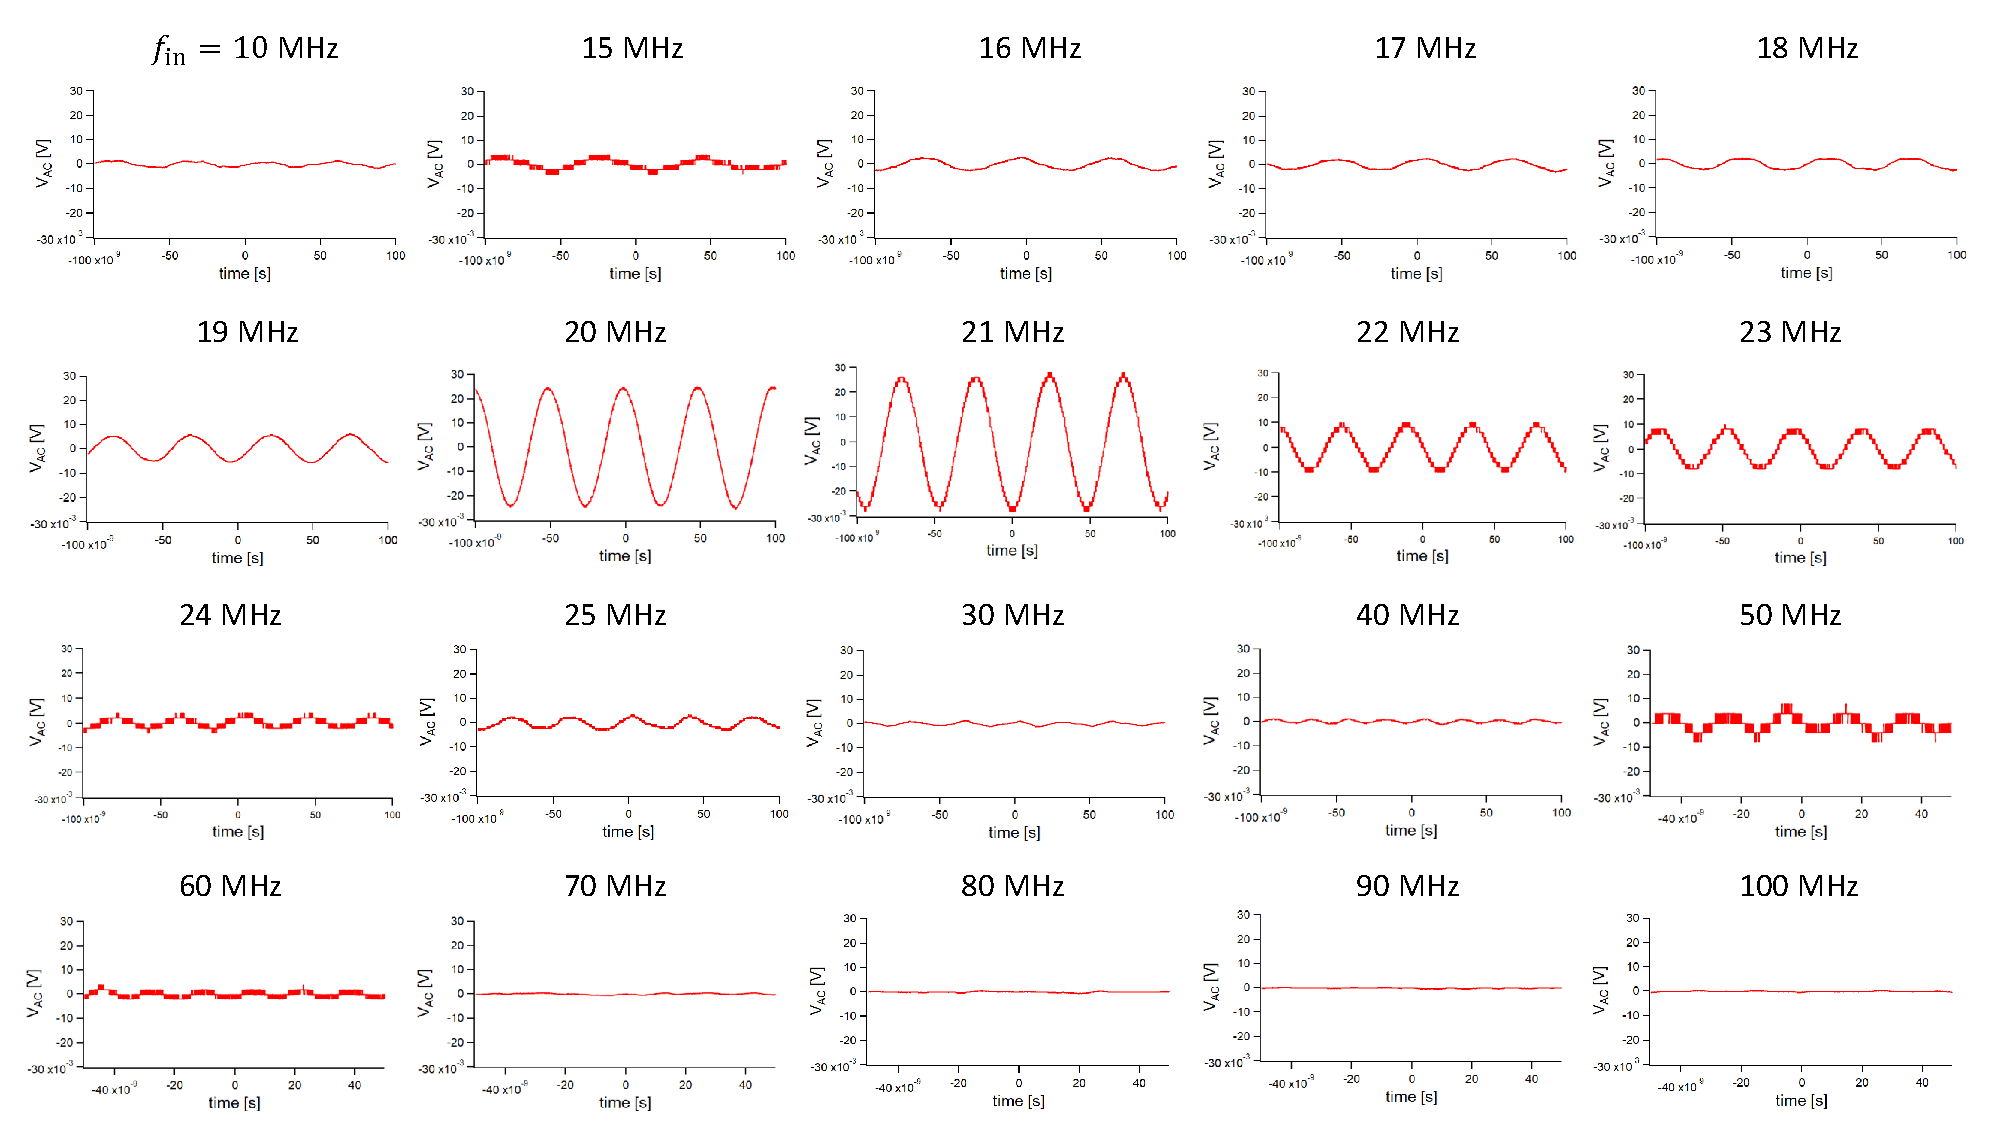
\includegraphics[width=15cm]{figure/3_5_detectorTest_LED.pdf}
	\caption{SRS検出器にLED光を入力した際のAC出力測定結果	\label{fig:DetectorTest_LED}}
\end{figure}

図\ref{fig:DetectorTest_laser}には検出器にレーザー光を入力した際のAC出力の測定結果を示す。
図\ref{fig:DetectorTest_laser}左のグラフは入射した変調光の波形を示す。
中央と右のグラフはそれぞれ、ND10、ND03のフィルターを用いて検出器前での変調光のパワーを調整した際のAC出力測定結果を示す。
図\ref{fig:DetectorTest_laser}より、検出器によるレーザー光の検出は確認できなかった。

\begin{figure}[H]
	\centering
	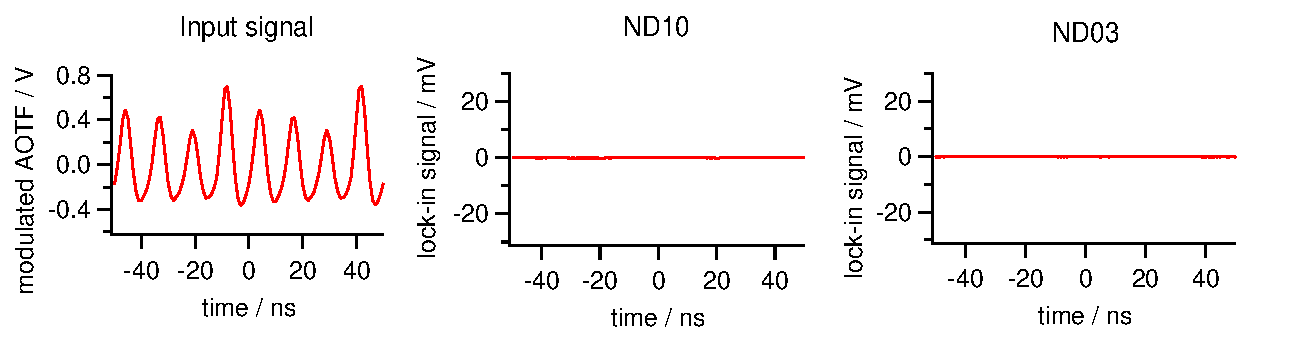
\includegraphics[width=15cm]{figure/3_6_detectorTest_laser.pdf}
	\caption{SRS検出器にレーザー光を入力した際のAC出力測定結果	\label{fig:DetectorTest_laser}}
\end{figure}

検出器のフォトダイオードを取り外し、電気信号を入力し、AC出力を測定した結果を図\ref{fig:DetectorTest_FG}に示す。
図\ref{fig:DetectorTest_FG}より、$f_{\mathrm{in}}=20$ MHzの時に検出器の出力が最大となっており、検出した周波数帯域は約10 MHzであった。\textcolor{red}{帯域はどうやって計算したのですか?}

\begin{figure}[H]
	\centering
	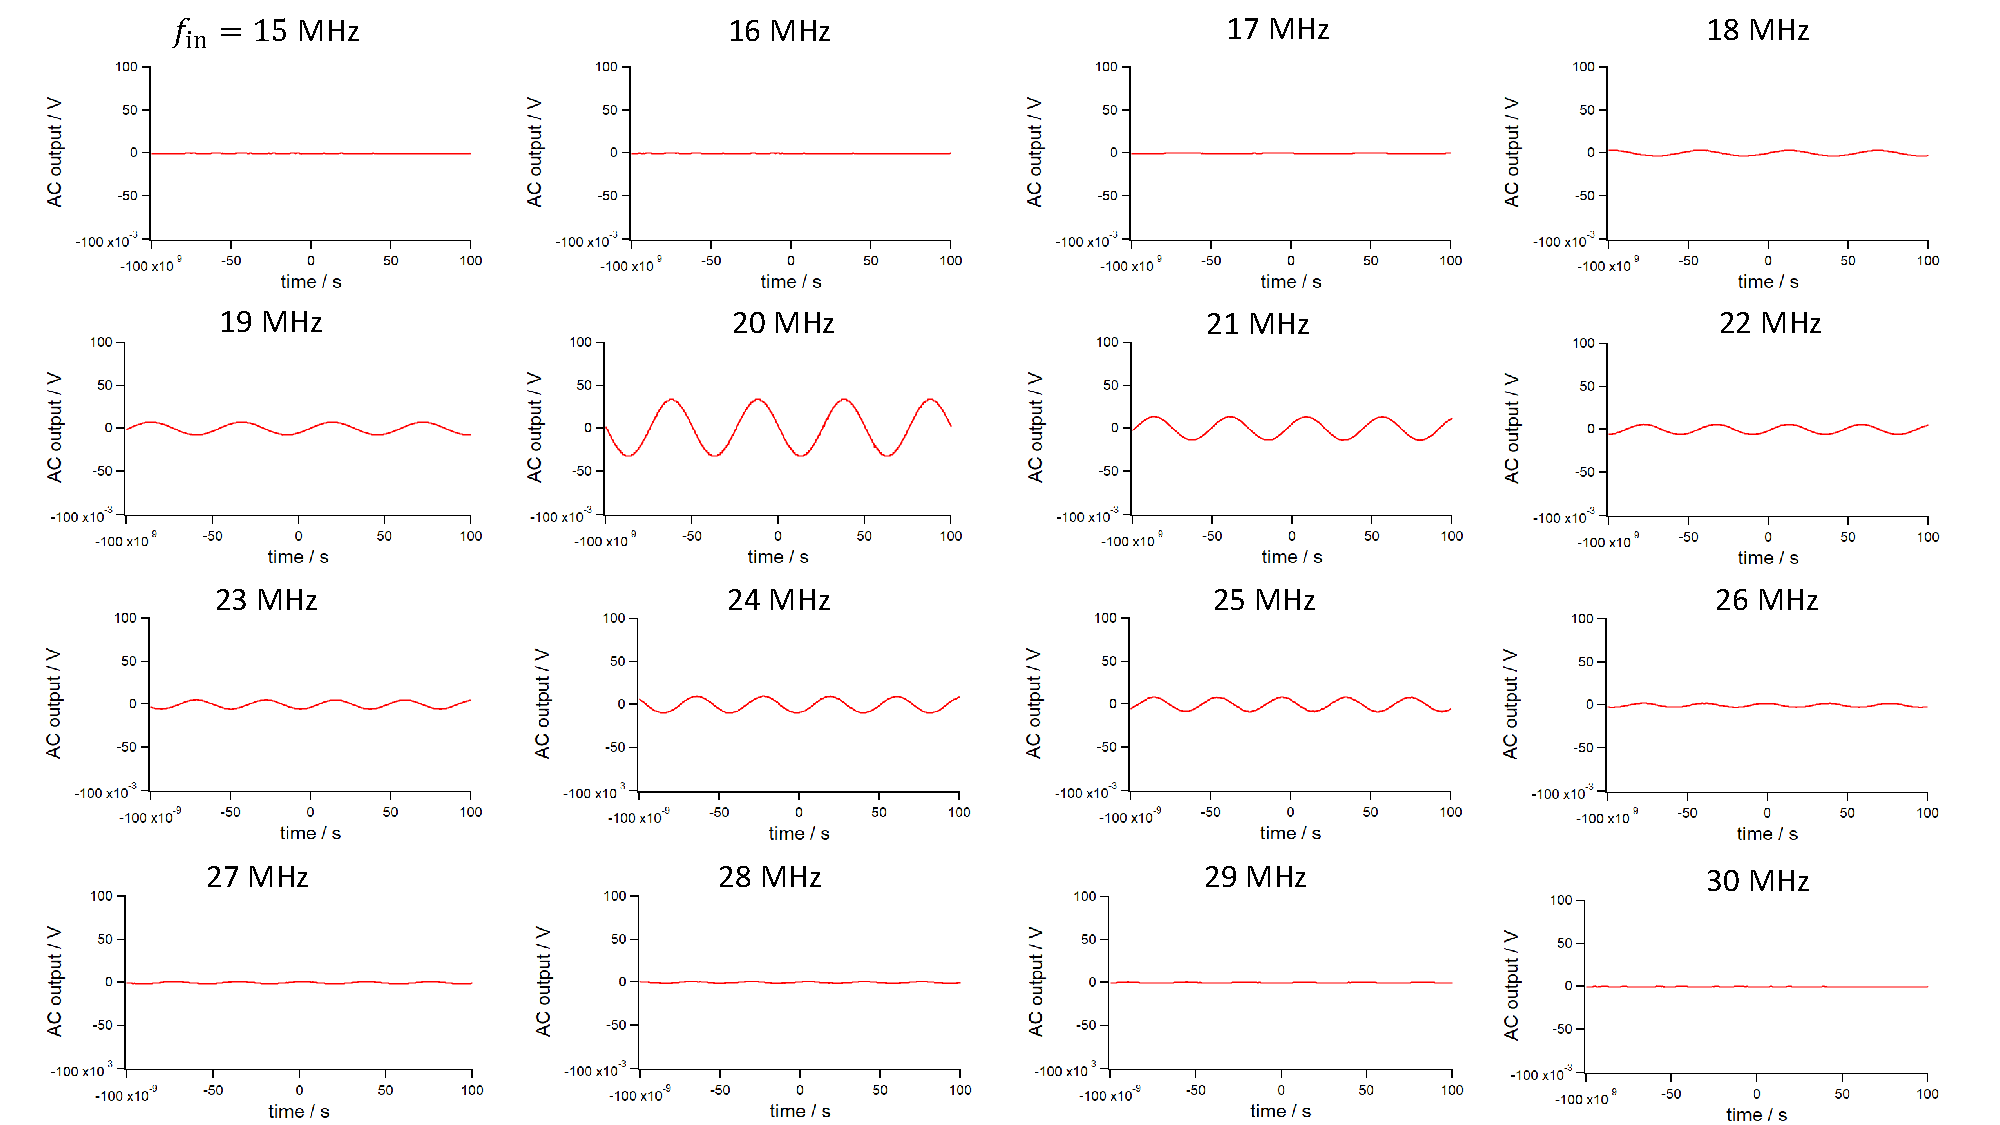
\includegraphics[width=15cm]{figure/3_7_detectorTest_FG.pdf}
	\caption{SRS検出器に電気信号を入力した際のAC出力測定結果	\label{fig:DetectorTest_FG}}
\end{figure}

\bibliography{reference} 
\bibliographystyle{junsrt} %引用順に記載

\end{document}